\subsection{Problemas de falta de información}

Se encontraron diferentes tipos de páginas que tenían grupos sin información e incluso páginas sin información alguna. A continuación se muestran varios ejemplos con los diferentes casos encontrados. %con falta de información.


\begin{itemize}
\item[-] Páginas en las cuales se tiene el nombre de la materia, pero no hay información de algún grupo: \url{http://www.fciencias.unam.mx/docencia/horarios/20081/1556/803}

\begin{figure}[H]
\centering
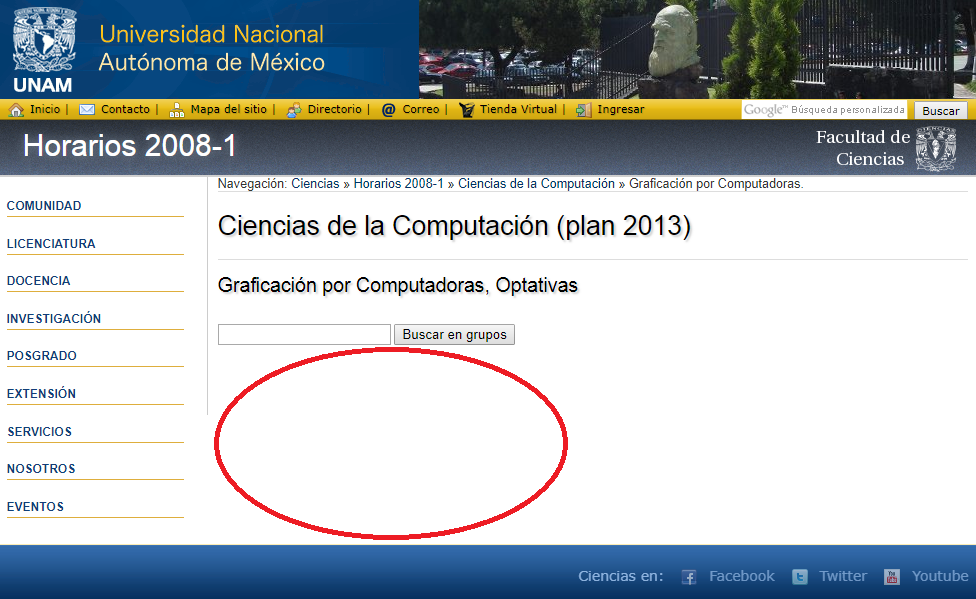
\includegraphics[scale = 0.45]{FaltaInfo_A} %width=\textwidth
\caption{\textit{Ejemplo de página web en blanco}}
\end{figure}

\item[-] Páginas que no tienen información del salón: \url{http://www.fciencias.unam.mx/docencia/horarios/20081/119/4}

\begin{figure}[H]
\centering
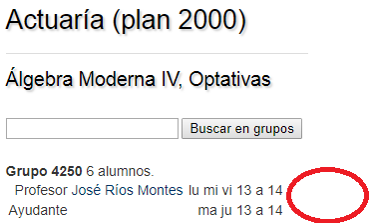
\includegraphics[scale = 0.45]{FaltaInfo_B} %width=\textwidth
\caption{\textit{Ejemplo de grupo sin información de salón}}
\end{figure}

\item[-] Páginas que tienen grupos sin información del número de alumnos inscritos en el grupo: \url{http://www.fciencias.unam.mx/docencia/horarios/20112/119/630}

\begin{figure}[H]
\centering
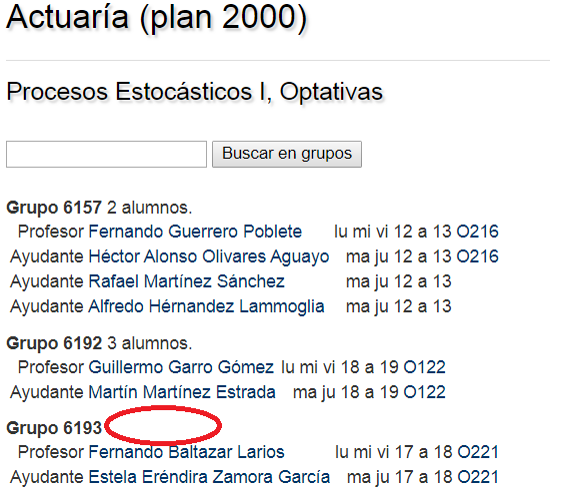
\includegraphics[scale = 0.6]{FaltaInfo_C} %width=\textwidth
\caption{\textit{Ejemplo de grupo sin información de alumnos}}
\end{figure}

\item[-] Páginas que tienen grupos sólo con el horario, sin nombre del profesor, salón, ayudante, número de alumnos, lugares disponibles: \url{http://www.fciencias.unam.mx/docencia/horarios/20091/119/841} \url{http://www.fciencias.unam.mx/docencia/horarios/20091/119/244}

\begin{figure}[H]
\centering
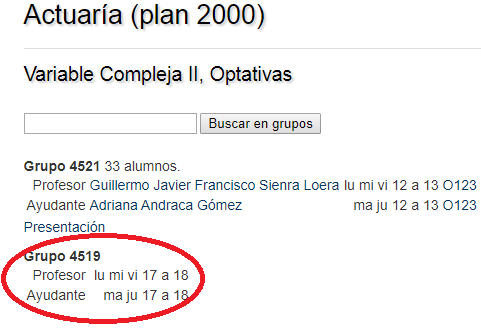
\includegraphics[scale = 0.8]{FaltaInfo_D} %width=\textwidth
\caption{\textit{Ejemplo de grupo sólo con horario}}
\end{figure}
\end{itemize}